\documentclass[17pt]{extarticle}
\usepackage{amsmath, amssymb}
\usepackage{nccmath}

\usepackage[a4paper, total={8in, 11.38in},top=2mm,left=27mm,bottom=2mm,right=2mm]{geometry}
\usepackage{tikz}
\usetikzlibrary{calc}
\usetikzlibrary{arrows.meta}
\usepackage{titlesec}


%% New Commands ----------------------------------
\newcommand{\pt}[1]{\draw (#1) circle(0.08);} %draw point 
%For example,  \pt {0,0}

%Extend to draw dot at midpint of segment
\newcommand{\dt}[2]{\draw ($(#1)!0.5!(#2)$) circle(0.08);\draw (#1)--(#2);}   %For example    \dt {0,0}{5,5};

%Extend to draw arrow at midpoint by combining two lines
\newcommand{\ma}[2]
{ \draw [shorten >= -2.5mm][-{Stealth[length=5mm]}] (#1) -- ($(#1)!0.5!(#2)$);  
 \draw ($(#1)!0.5!(#2)$)--(#2);  
}
%%%End of new commands-----------------------------

\titleformat{\section}
{\normalfont\normalsize\bfseries}{\thesection}{1em}{}

\titleformat{\subsection}
{\normalfont\normalsize\bfseries}{\thesection}{1em}{}

\begin{document}

\noindent
\begin{fleqn} 

%%%%%%%%%%%%%%%%%%%%%%%%%%%%%%%%%%%%%%%%%%%%%%%%%%%%%%%%%%%%%%%%

\section{Question}
Show by vector method that the sum of the squares of the diagonals of a parallelogram is equal to the sum of the squares of its sides.
%----------------------------------------
\subsection*{Answer}
$\text{Let ABCD be a parallelogram with }$ \\
$\overline{AB} = \overline{DC} = \overline{a} \text{\;\;\;and}$\\
$\overline{BC} = \overline{AD} = \overline{b}$\\
\vspace{-0.5cm}
\begin{equation} \nonumber
\begin{alignedat}{4}
&\text{LHS } \\&= AC^2+BD^2 \\
&= |\overline{AC}|^2 + |\overline{BD}|^2\\
&= |\overline{AB}+\overline{BC}|^2 + |\overline{BC}+\overline{CD}|^2\\
&= |\overline{a}+\overline{b}|^2 + |\overline{a}-\overline{b}|^2\\
&= (\overline{a}+\overline{b})\cdot (\overline{a}+\overline{b})+(\overline{a}-\overline{b})\cdot(\overline{a}-\overline{b})\\
&= |\overline{a}|^2 + 2\overline{a} \cdot \overline{b}+|\overline{b}|^2 +|\overline{a}|^2 - 2\overline{a} \cdot \overline{b}+|\overline{b}|^2 
\end{alignedat}
%\vrule
%\vspace{1cm}
\begin{alignedat}{4}
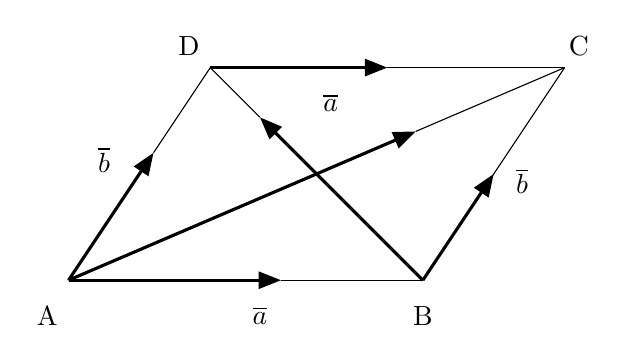
\begin{tikzpicture}[scale=0.9]
\draw[-{Stealth[inset=0mm]},line width=0.4mm] (0,0) -- (1.2,1.8);
\draw (1.2,1.8) -- (2,3); 
\draw[-{Stealth[inset=0mm]},line width=0.4mm] (2,3) -- (4.5,3);
\draw (4.5,3) -- (7,3);

\draw (5.8,1.2)--(7,3);
\draw [-{Stealth[inset=0mm]},line width=0.4mm] (5,0) -- (6,1.5);

\draw [-{Stealth[inset=0mm]},line width=0.4mm] (0,0) -- (3,0);
\draw (3,0) -- (5,0);

%Two Cross line segments only partial 
\draw [-{Stealth[inset=0mm]},line width=0.4mm] (0,0)--(4.9,2.1);
\draw (4.9,2.1) -- (7,3);

\draw [-{Stealth[inset=0mm]},line width=0.4mm] (5,0)--(2.7,2.3);
\draw (2.7,2.3) -- (2,3);

\node at (0.5,1.7){$\overline{b}$};
\node at (6.4,1.4){$\overline{b}$};
\node at (3.7,2.5){$\overline{a}$};
\node at (2.7,-0.5){$\overline{a}$};
\node at (-0.3,-0.5){A};
\node at (5,-0.5){B};
\node at (1.7,3.3){D};
\node at (7.2,3.3){C};
\end{tikzpicture}
\\ \    % Only space charachter after several newlines to raise the figure
\end{alignedat}
\end{equation}
\vspace{-0.2cm}
\begin{equation} \nonumber
\begin{alignedat}{4}
&= |\overline{a}|^2 + |\overline{b}|^2 +|\overline{a}|^2 +|\overline{b}|^2  \\
&= |\overline{AB}|^2 + |\overline{BC}|^2 +|\overline{CD}|^2 +|\overline{DA}|^2  \\
\end{alignedat}
\quad
\vrule
\quad
\begin{alignedat}{4}
&= \overline{AB}^2 + \overline{BC}^2 +\overline{CD}^2 +\overline{DA}^2 \\ &= \text{RHS}
\end{alignedat}
\end{equation}


%%%%%%%%%%%%%%%%%%%%%%%%%%%%%%%%%%%%%%%%%%%%%%%%%%%%%%%%%%%%%%%%

\section{Question}
Prove using vector method that the angle subtended on a semi-circle is a right angle.
%----------------------------------------

\subsection*{Answer}

\begin{equation} \nonumber
\begin{alignedat}{4}
\begin{minipage}{15em}
  Consider a semicircle on a diameter AB with center O and radius r. Let C be any point on the circle other than A or B. \\ \\Let $\overline{a}, \overline{b}, \overline{c}$ be the position vectors of the point A, B and C respectively.
  \end{minipage}
\end{alignedat}
%\vrule
\quad\quad\quad
\begin{alignedat}{4}
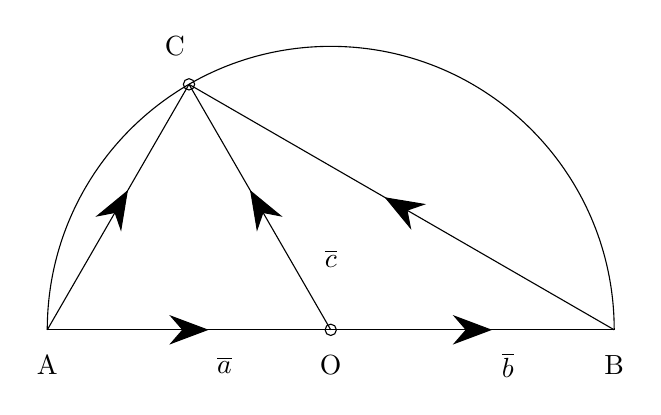
\begin{tikzpicture}[scale=0.9]
%\draw[very thin, gray!40, step=1 cm](0,0) grid (8,5);
\draw (0:8) arc (0:180:4);
\pt {4,0};
\ma {0,0}{4,0};
\pt {2,{sqrt(12))}}; %% take a point on the circle say ( 2,sqrt(12) )
                     %% calculated by calc packageS
\ma {4,0}{2,{sqrt(12))}};
\ma {8,0}{2,{sqrt(12))}};
\ma {0,0}{2,{sqrt(12))}};
\ma {4,0}{8,0};
\node at (0,-0.5){A};
\node at (4,-0.5){O};
\node at (1.8,4){C};
\node at (8,-0.5){B};

\node at (2.5, -0.5){$\overline{a}$};
\node at (6.5,-0.5){$\overline{b}$};
\node at (4,1){$\overline{c}$};


\end{tikzpicture}\\\
\end{alignedat}
\end{equation}
\begin{equation} \nonumber
\begin{alignedat}{4}
\text{Then }\\
 \overline{AC} \cdot \overline{BC} &= 
             (\overline{c} - \overline{a}) \cdot  
             (\overline{c} - \overline{b})\\
&= (\overline{c} - \overline{a}) \cdot  
             (\overline{c} + \overline{a}) 
            \quad \boxed { \;-\overline{b}=\overline{a}\;}\\
&= |\overline{c}|^2 - |\overline{a}|^2 \\
&= r^2 - r^2 = 0 \\
\end{alignedat}
\quad
\vrule
\quad
\begin{alignedat}{4}
& \therefore \; \overline{AC} \perp \overline{BC}\\
& \therefore \; \text{Seg AB} \perp \text{Seg BC}\\
& \therefore \; \text{Angle in Semi-circle}\\
& \therefore \; \text{is right angle.} 
\end{alignedat}
\end{equation}
%%%%%%%%%%%%%%%%%%%%%%%%%%%%%%%%%%%%%%%%%%%%%%%%%%%%%%%%%%%%%%%%

\end{fleqn}
\end{document} 